\subsection{Trainierung des Modells}
\label{sec:Trainierung}
Für die Trainierung werden zunächst noch zwei Callbacks definiert, um den Trainingsprozess zu verbessern.
Callbacks sind Funktionen, die nach jeder Epoche des Trainings aufgerufen werden.
Diese erhalten das Modell bei jedem Aufruf in seinem momentanen Zustand.
Daraufhin können Callbacks das Modell beispielsweise auf Testdaten anwenden, die Parameter des Trainings verändern oder das Training beenden.
Ein hilfreicher Callback ist \emph{EarlyStopping}.
Dieser überwacht die Performance des Modells mithilfe einer beliebigen Metrik und beendet das Training, wenn sich die Metrik nicht mehr signifikant verbessert \cite{KerasEarlyStopping}.
Somit kann überflüssige Trainingszeit gespart und Überanpassung vermieden werden.
Die Definition des Callbacks ist in \autoref{lst:ModelTraining} in Zeile 1 und 2 zu sehen.

\begin{code}
\begin{minted}[
    linenos,
    numbersep=10pt,
    gobble=0,
    frame=lines,
    framesep=2mm,
    escapeinside=!!]{python}
early_stopping = keras.callbacks.EarlyStopping(monitor="val_loss",
    patience=10, restore_best_weights=True)
reduce_lr = keras.callbacks.ReduceLROnPlateau(monitor="val_loss", patience=5)

epochs = 32
batch_size = 12
!\label{fit_start}!history = model.fit(
    x_train, y_train,
    batch_size=batch_size, epochs=epochs,
    validation_data=(x_val, y_val),
!\label{callbacks_passing}!    callbacks=[early_stopping, reduce_lr]
!\label{fit_end}!)
\end{minted}
\captionof{listing}{Definition der Callbacks zur Verbesserung des Trainings und Trainierung des Modells}
\label{lst:ModelTraining}
\end{code}

Die überwachte Metrik ist der Verlustwert der Validierung.
Der Parameter \emph{patience} bestimmt, wie viele Epochen ohne eine verbesserung der überwachten Metrik gewartet werden sollen, bis das Training beendet wird.
Die in Zeile 2 aktivierte Option \emph{restore\_best\_weights} besagt, dass das Modell am Ende des Trainings in den Zustand gebracht werden soll, bei dem die überwachte Metrik den besten Wert hatte.
Dies kann beispielsweise Sinnvoll sein, wenn sich der Verlustwert der Validierung durch Überanpassung gegen Ende wieder verschlechtert.
Allerdings muss diese Option mit Vorsicht verwendet werden, da sie auch eine Überanpassung an die Validierungsdaten begünstigt.

Ein weiterer hilfreicher Callback ist \emph{ReduceLROnPlateau}.
Dieser Callback verringert die Lernrate, wenn sich eine bestimmte Metrik nicht weiter verbessert \cite{KerasReduceLROnPlateau}.
Dies hat dann zur Folge, dass die Parameter des Modells noch etwas weiter optimiert werden können.
In \autoref{lst:ModelTraining} wird dieser Callback in Zeile 3 definiert.
Auch hier wird der Verlustwert der Validierung überwacht.
Ähnlich wie bei \emph{EarlyStopping} bestimmt der Parameter \emph{patience} hier, nach wie vielen Epochen ohne eine Verbesserung der überwachten Metrik die Lernrate verringert wird.
Dieser Wert muss kleiner sein als der von \emph{EarlyStopping}, damit der Callback einen Effekt hat.
In Zeile \ref{callbacks_passing} werden die Callbacks schließlich an \emph{model.fit()} übergeben, wodurch sie bei der Trainierung angewendet werden.

Als Nächstes müssen noch die maximale Anzahl an Trainingsepochen und die Stapelgröße (engl. \emph{batch size}) ausgewählt werden.
Die maximale Anzahl an Trainingsepochen kann großzügig gewählt werden, da das Training letztendlich vom \emph{EarlyStopping}-Callback beendet werden soll.
Wird das Training davor durch die maximale Anzahl an Trainingsepochen beendet, bleibt eventuelles Potenzial ungenutzt.
Für das hier verwendete Modell ist eine maximale Anzahl an Trainingsepochen von 32 angemessen.
Die Stapelgröße hingegen ist ein kritischer Parameter.
Je größer die Stapelgröße ist, desto schneller verläuft das Training, da der gesamte Stapel parallel verarbeitet wird.
Jedoch muss der gesamte Stapel in den Arbeitsspeicher passen.
Besonders unter Verwendung einer \acrshort{gpu} ist der Arbeitsspeicher jedoch stark limitiert, da das Modell mit dem Stapel komplett in den Speicher der \acrshort{gpu} passen muss.
Die Stapelgröße sollte also so gewählt werden, dass der Speicher bestmöglich ausgefüllt wird.
Da die Trainingsdaten im vorliegenden Anwendungsfall größer sind als bei einfachen Klassifizierungsaufgaben, kann die Stapelgröße nicht sehr groß gewählt werden.
Bei einer Stapelgröße von 12 reicht der 8 GB große Speicher der verwendeten Grafikkarte \emph{Nvidia GeForce GTX 1080} gerade aus.

Nun da die notwendigen Hyperparameter definiert sind, kann das Modell trainiert werden.
Dazu wird \emph{model.fit()} aufgerufen, wie in \autoref{lst:ModelTraining} in Zeile \ref{fit_start} bis \ref{fit_end} gezeigt.
Diese Methode gibt die Entwicklung verschiedener Metriken im Verlauf des Trainings zurück.
Auf der oben erwähnten Grafikkarte dauert das Training pro Epoche ca. 80 Sekunden.
Nach 26 Epochen beendet der \emph{EarlyStopping}-Callback das Training, insgesamt dauert das Training also ca. 35 Minuten.
Der Verlauf des Verlustwerts ist in \autoref{fig:TrainingLoss} dargestellt.

\begin{figure}[h]
    \centering
    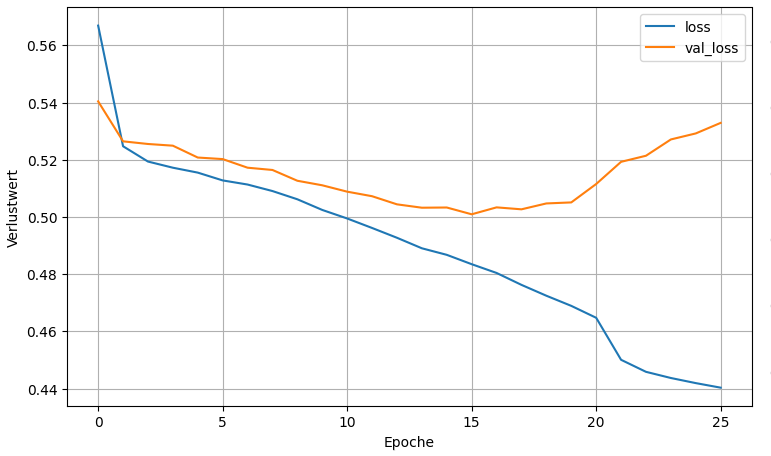
\includegraphics[width=0.8\textwidth,height=8cm,keepaspectratio=true]{content/images/TrainingLoss.png}
    \caption{Entwicklung des Verlustwerts über die Epochen des Trainings}
    \label{fig:TrainingLoss}
\end{figure}

In der Abbildung ist zunächst erkennbar, dass der Verlustwert über die Epochen hinweg optimiert werden kann.
Ab der 15. Epoche beginnt der Verlustwert der Validierung jedoch anzusteigen, während der Verlustwert des Trainings weiter sinkt.
Dieser Effekt spricht für eine Überanpassung.
Dies bedeutet, dass das Modell ab einer bestimmten Epoche beginnt, die Trainingsdaten "`auswendig"' zu lernen.
Dadurch handelt das Modell bei der Validierung jedoch nicht mehr nach den globalen Mustern, wodurch die Vorhersagen anhand der Validierungsdaten schlechter werden.
Der \emph{EarlyStopping}-Callback stellt jedoch den besten Zustand des Modells wieder her, der in diesem Fall bei Epoche 15 bestand.
